\section{Catmull-Clark}

\subsection{Allgemein}

Der Catmull-Clark Algorithmus wurde 1978 von Edwin Catmull und James Clark entwickelt.
Er ist eine Verallgemeinerung von bi-cubic uniform B-splines surfaces und arbeitet auf
Netzen mit beliebiger Topologie.
Das neu erzeugte Netz ist immer ein Vierecksnetz. Jedes n-Gon im Eingabenetz wird in n Quads
im Ausgabenetz umgewandelt.
Die Kontrollpunkte des Netzes werden durch Unterteilung approximiert.


\subsection{Unterteilungsregeln}

\begin{figure}
\centering
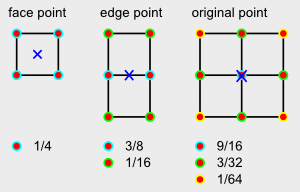
\includegraphics[width=0.6\textwidth]{content/media/sd_catmull_mask.png}
\caption{Catmull-Clark Maske \cite{yoshihitoyagi.23.12.2015}}
\label{fig:sd_catmull_mask}
\end{figure}

\cite{rosettacode.23.12.2015}
\cite{rorydriscoll.23.12.2015}
\cite{yoshihitoyagi.23.12.2015}



\subsection{Sonderfälle}


